%% ****** Start of file apstemplate.tex ****** %
\documentclass[aps,prl,reprint,groupedaddress]{revtex4-2}

% You should use BibTeX and apsrev.bst for references
% Choosing a journal automatically selects the correct APS
% BibTeX style file (bst file), so only uncomment the line
% below if necessary.
% \bibliographystyle{apsrev4-2}

\usepackage{graphicx}
\usepackage{epstopdf}
\usepackage{amsmath}
\usepackage{amsthm}
\usepackage{amsfonts}
\usepackage{subfigure}
\usepackage{hhline}
\usepackage[left=1cm,right=1cm,top=1cm,bottom=1cm]{geometry}
\usepackage[miktex]{gnuplottex}
\usepackage{xcolor}
\usepackage{amssymb}
\usepackage{amsmath}
\usepackage{color}
\usepackage{hyperref}
\usepackage[percent]{overpic}
\usepackage{tikz}
\usepackage{mathrsfs}
\usepackage{wasysym}
\usepackage{tikz-cd}
\usepackage{caption}  % Elimina hypcap=true si está presente
\usepackage{stackengine,scalerel}

\usepackage{caption}
\captionsetup{skip=0pt}  % Reduce el espacio entre la imagen y su caption
\raggedbottom

% so sections, subsections, etc. become numerated.
\setcounter{secnumdepth}{3}

\newenvironment{Figura}
  {\par\medskip\noindent\minipage{\linewidth}}
  {\endminipage\par\medskip}

\renewcommand{\appendixname}{Apéndice} % Change "Appendix" to "Apéndice"

\begin{document}

%Title of paper
\title{
Fashion-MNIST con PyTorch
}

% autores
\author{Kevin Gaston Mansilla}
\email[]{kevin.mansilla@mi.unc.edu.ar}

\affiliation{}

%fecha
\date{\today}

\begin{abstract}
\end{abstract}

% insert suggested keywords - APS authors don't need to do this
%\keywords{}

%\maketitle must follow title, authors, abstract, and keywords
\maketitle

\section{Introducción}
Las redes feed forward son un tipo de red neuronal que estan compuestas por 
$N$ capas donde $N-1$ son capas ocultas. La primera capa no se contabiliza 
porque es la capa de entrada, la particularidad de estas redes es que las 
conexiones se realizan entre capas consecutivas, es decir, no hay conexiones
entre capas no consecutivas, como lo muestra la Figura \ref{fig-feed-forward}.
\begin{Figura}
  \centering
  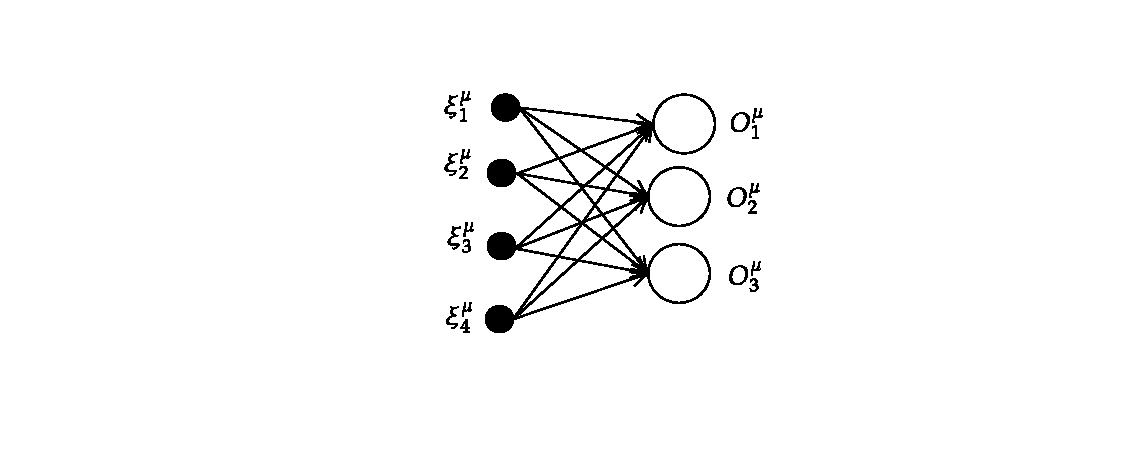
\includegraphics[width=1\textwidth]{figs/red-feed-forward.pdf}
  \captionof{figure}{Red feed forward}
  \label{fig-feed-forward}
\end{Figura}

Puede computarse la salida de la red mediante la siguiente ecuación:
\begin{equation}
  O^{\mu}_{i} = g(h_{i}) - g \left( \sum_{k} w_{ik} \xi_{k} \right)
  \label{eq-feed-forward}
\end{equation}

En la ecuación \ref{eq-feed-forward}, la relación o conexiones entre las neuronas 
de entrada ($\xi_{k}$) y las neuronas de salida ($O^{\mu}_{i}$) se representa por 
medio de los ponderadores $w_{ik}$, donde $i$ es el índice de la neurona de salida 
y $k$ es el índice de la neurona de entrada. El cáculo de la salida dependera 
de la función de activación $g$ y de la función de propagación $h_{i}$.

Al utilizar una red feed forward autoencoder, se busca que la red aprenda a
reconstruir la entrada en la salida, es decir, que la salida sea igual a la entrada.
Por lo tanto, la red debe aprender a comprimir la información de entrada en una
representación más pequeña, para luego descomprimir la información y obtener la
salida. Como trabajaremos con una solo capa oculta, la red tendrá la
arquitectura de la figura \ref{fig-feed-forward-autoencoder}, donde $V_{j}$ 
es la función de activación de la capa oculta.

\begin{Figura}
  \centering
  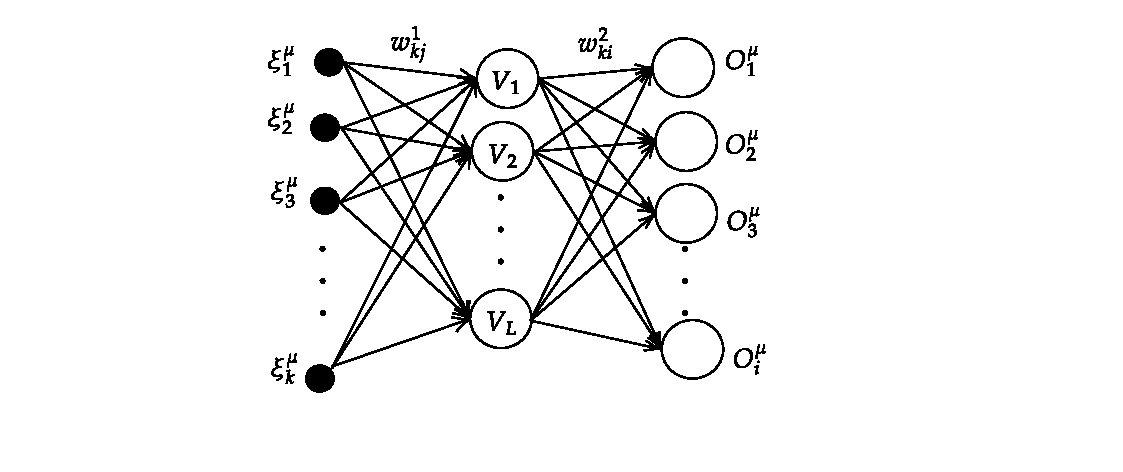
\includegraphics[width=1\textwidth]{figs/red-autoencoder.pdf}
  \captionof{figure}{Red feed forward autoencoder}
  \label{fig-feed-forward-autoencoder}
\end{Figura}

Este tipo de redes, tienen la particularidad que la capa de entrada y la capa 
de salida deben tener la misma cantidad de neuronas, mientras que las capas 
intermedias deben tener una cantidad menor de neuronas. Esto obliga a la red a 
encontrar patrones entre los elementos de entrada y salida, de forma que aprenda 
a presentar la información comprimida y permitiendo asi reducir la dimensionalidad 
de los datos. 

\section{Arquitectura de Red Neuronal}
En este trabajo, se implementará una red feed forward autoencoder al corpus 
Fashion-MNIST, el cual consiste en un conjunto de imágenes de ropa en escala de
grises de 28x28 pixeles, conformadas por:
\begin{verbatim}
0: 'T-shirt/top',
1: 'Trouser',
2: 'Pullover',
3: 'Dress',
4: 'Coat',
5: 'Sandal',
6: 'Shirt',
7: 'Sneaker',
8: 'Bag',
9: 'Ankle boot'
\end{verbatim}

Donde el principal objetivo es clasificar una imagen de entrada en una de las 
$10$ categorías. En la figura \ref{fig-red} se muestra la arquitectura de la red.
Donde se observa que a la imagen inicial en la capa $1$ se la aplica un 
\textit{flatten} para transformar la imagen de $28x28$ en un vector de $784$ 
elementos, luego pasa por la primera capa oculta de $n1$ neuronas la cual al 
inicio se le aplica un modulo \textit{lineal}, luego se le aplica una función 
de activación \textit{ReLU} y finalmente se le aplica un modulo \textit{dropout} 
con una probabilidad de $0.2$.

Luego, la salida de la primera capa oculta pasa por la segunda capa oculta de $n2$
neuronas que tiene el mismo comportamiento que la primera capa oculta. Finalmente,
el flujo de la red llega a la capa final que tiene $10$ neuronas cada una 
representando una de las categorías de Fashion-MNIST. Asi el output final es un 
vector de $10$, en este ejemplo particular se puede ver que como input se paso 
una imagen de Ankle boot y como el output el valor más alto se da en la posición
$9$ significa que la red clasifico correctamente la imagen.

\begin{Figura}
  \centering
  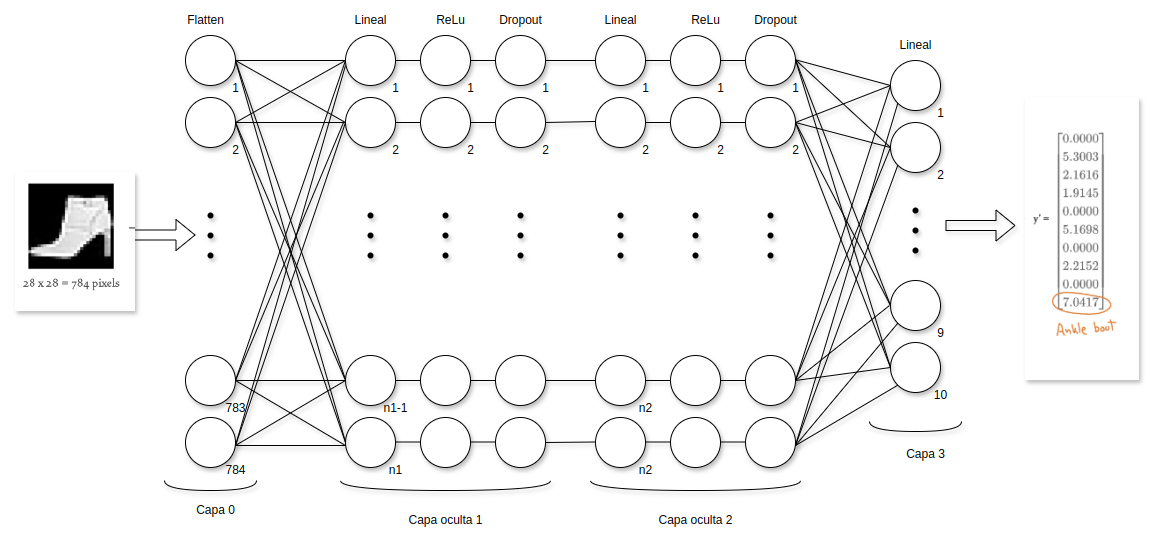
\includegraphics[width=1\textwidth]{figs/arq_model.png}
  \captionof{figure}{Arquitectura de la red neuronal}
  \label{fig-red}
\end{Figura}

Entonces el objetivo del trabajo sera entrenar esta red usando PyTorch como 
función de pardida se utiliza el error cuadrático medio y el método de descenso 
por el gradiente estocástico como algoritmo de optimización (minimización), 
con un learning rate de $1e-3$ que indica 'de que tamaño' dar el paso 
para que el algoritmo converga a la solución. Lo idear es hacerlo de forma 
proporcional al gradiente, es decir, si el gradiente es grande el paso será
grande y si el gradiente es pequeño el paso será pequeño.

El proceso de descenso por el gradiente estocástico se realiza en mini-batches,
es decir, se toma un subconjunto de los datos de entrenamiento y se calcula el
gradiente para ese subconjunto, luego se actualizan los pesos de la red y se
toma otro subconjunto de datos y se repite el proceso. Esto se hace para evitar
que la red se sobreajuste a los datos de entrenamiento y no pueda generalizar
a datos nuevos.

Como base se utilizaran los siguientes hiperparámetros: $n1=128$, $n2=64$, 
$30$ épocas y un batch size de $100$ con un optimizador 
Stoachastic Gradient Descent (SGD) con un learning rate de $1e-3$. Luego se 
realizaran pruebas variando los hiperparámetros para ver como afectan al 
desempeño de la red, en particular se cambiara el optimizador por Adam y 
por ultimo se cambiara las epocas a $60$, en la siguiente sección presentaremos
estos resultados

\section{Resultados}

Aqui presentaremos los resultados obtenidos al entrenar la red neuronal en los 
diferentes modelos planteados. Los hiperparámetros son:

\begin{itemize}
  \item Modelo 1: $n1=128$, $n2=64$, $30$ épocas y un batch size de $100$ con un
  optimizador Stoachastic Gradient Descent (SGD) con un learning rate de $1e-3$.
  \item Modelo 2: $n1=128$, $n2=64$, $30$ épocas y un batch size de $100$ con un
  optimizador Adam con un learning rate de $1e-3$.
  \item Modelo 3: $n1=128$, $n2=64$, $60$ épocas y un batch size de $100$ con un
  optimizador Adam con un learning rate de $1e-3$.
\end{itemize}

En la tabla \ref{tab:models} se presentan los resultados obtenidos para cada
modelo. Donde se puede observar que el modelo 2 y 3 tienen un mejor desempeño
que el modelo 1, esto se debe a que el optimizador Adam es más eficiente que el
SGD, ya que este último no tiene en cuenta la dirección del gradiente, sino que
se mueve en la dirección opuesta al gradiente. Por otro lado, se observa que el
el modelo 2 y el 3 tienen un desempeño similar, lo que significa que aumenta 
las epocas de entrenamiento no necesariamente mejora el desempeño de la red.

Entonces, se puede concluir que el modelo 2 es el mejor modelo, ya que tiene un
mejor desempeño y menor tiempo de entrenamiento que el modelo 3.

\begin{table}[h!]
  \begin{tabular}{lccll}
    \hline
    Modelos   & Loss      & Acuracy  & \\ \hline
    Modelo 1  & $0.51\% $ & $81.0\%$ & \\
    Modelo 2  & $0.32\% $ & $89.3\%$ & \\
    Modelo 3  & $0.37\% $ & $89.1\%$ & \\ \hline
  \end{tabular}
  \caption{Resultados del entrenamoento de la red neuronal}
  \label{tab:models}
\end{table}

\subsection{Modelo Base}

\subsection{Modelo con optimizador Adam}

\subsection{Modelo con 60 épocas}



\section{Conclusiones}

\bibliography{ref}

% Specify following sections are appendices. Use \appendix* if there
% only one appendix.

%\onecolumngrid


\end{document}
%
% ****** End of file apstemplate.tex ******